\chapter{Szenario}

Im Wesentlichen sollen die hier besprochenen Algorithmen in einem \"Uberwachungsszenario getestet werden, d.h. die Qualit\"at eines Algorithmus wird anhand des Anteils der Zeit bewertet, die er das Zielobjekt \"uberwachen konnte, relativ zur Gesamtzeit. 

Verwendetes Umfeld wird ein quadratischer Torus sein, der aus quadratischen Feldern besteht.
Jedes bewegliche Objekt auf einem Feld kann sich nur auf eines der vier Nachbarfelder bewegen oder stehenbleiben. 
Die Felder k\"onnen entweder leer oder durch ein Objekt besetzt sein. Besetzte Felder k\"onnen nicht betreten werden. Es gibt drei verschiedene Arten von Objekten, unbewegliche Hindernisse, ein zu \"uberwachende Zielagent und Agenten. Zielagent und Agent bewegen sich anhand eines bestimmten Algorithmus anhand bestimmter Sensordaten.

TODO Aufl\"osen

\section{Problem-Instanzen}

Eine einzelne Probleminstanz entspricht einem Torus mit einer (abh\"angig vom verwendeten Random-Seed-Wert) bestimmten Anfangsbelegung mit bestimmten Objekten und bestimmten Parametern zur Sichtbarkeit. Die Parameter bestimmen, ob und wie Objekte andere Objekte die Sicht versperren und bis zu welcher Distanz der Zielagent von einem Agenten als ``\"uberwacht'' gilt, sofern die Sicht durch andere Objekte nicht versperrt ist.

Ein Experiment entspricht dem Test einer Anzahl von Probleminstanzen mit einer Reihe von Random-Seed-Werten.
In einem Durchlauf werden mehrere Experimente (jeweils mit unterschiedlichen Random-Seed-Wert-Reihen) durchgef\"uhrt.

\section{Qualit"at}

Problem-Qualit\"at eines Algorithmus zu einem Problem wird anhand des Anteils der Zeit berechnet, die er das Zielobjekt w\"ahrend des Problems \"uberwachen konnte, relativ zur Gesamtzeit. 
Experiment-Qualit\"at eines Algorithmus zu einer Anzahl von Problemen (einem Experiment) wird Anhand des Gesamtanteilder Zeit berechnet, die er das Zielobjekt w\"ahrend aller Probleme \"uberwachen konnte, relativ zur Gesamtzeit aller Probleme.
Qualit\"at eines Algorithmus entspricht dem Durchschnitt aller Experimentqualit\"aten des Algorithmus.

Halbzeit-Problem-Qualit\"at eines Algorithmus zu einem Problem entspricht dem Anteil der Zeit, die der Algorithmus das Zielobjekt w\"ahrend jeweils der zweiten H\"alfte des Problems \"uberwachen konnte, relativ zur halben Gesamtzeit.
Halbzeit-Experiment-Qualit\"at eines Algorithmus zu einer Anzahl von Problemen entspricht dem Anteil der Zeit, die der Algorithmus das Zielobjekt w\"ahrend jeweils der zweiten H\"alfte des Problems \"uberwachen konnte, relativ zur halben Gesamtzeit aller Probleme.
Die Halbzeitqualit\"at eines Algorithmus entspricht dem Durchschnitt aller Halbzeit-Experiment-Qualit\"aten eines Algorithmus.







\chapter{Agenten}

\section{Sensoren}

Jeder Agent besitzt 3 Gruppen mit jeweils 4 Bin\"arsensoren. Alle Sensoren sind visuelle Sensoren mit begrenzter Reichweite. Je nach Parameter des Szenarios wird die Sicht durch andere Objekten blockiert. Sichtlinien werden durch einen einfachen Bresenham-Linienalgorithmus bestimmt.
Jede Gruppe von Sensoren nimmt einen anderen Typ von Objekt wahr. Die erste Gruppe nimmt den Zielagenten, die zweite andere Agenten und die dritte Hindernisse.
Ein Sensor ist jeweils in eine bestimmte Richtung ausgerichtet (Norden, Osten, S\"uden, Westen) und wird auf ``wahr'' gesetzt, wenn sich in dem von der Sichtweite bestimmten Kegel ein entsprechendes Objekt befindet.

\section{F\"ahigkeiten}

Jeder Agent kann in jedem Schritt zwischen 5 verschiedenen Aktionen w\"ahlen, die den vier Richtungen plus einer Aktion, bei der der Agent sich nicht bewegt, entsprechen. Agenten k\"onnen pro Zeiteinheit genau einen Schritt durchf\"uhren. Der Zielagent kann je nach Szenario mehrere Schritte ausf\"uhren.
K\"onnte der Zielagent ebenfalls nur einen Schritt ausf\"uhren, w\"are das Problem sehr simpel, da der Zielagent Schwierigkeiten h\"atte, Agenten abzusch\"utteln, deren einzige Strategie es ist, sich in Richtung des Zielagenten zu bewegen.

\section{Ablauf der Bewegung}
Alle Agenten werden nacheinander in der Art abgearbeitet, dass der jeweilige Agent die aktuellen Sensordaten aus der Umgebung holt und anhand dieser die n\"achste Aktion bestimmt. Ung\"ultige Aktionen, d.h. der Versuch sich auf ein besetztes Feld zu bewegen, schlagen fehl und der Agent f\"uhrt in diesem Schritt keine Aktion aus, wird aber nicht weiter bestraft. Eine detaillierte Beschreibung wird in Kapitel~\ref{conclusion:cha} geliefert.

\section{Grunds\"atzliche Algorithmen der Agenten}

Neben denjenigen Algorithmen die auf LCS basieren und weiter untern besprochen werden, gibt es folgende Grundtypen, die dazu dienen, die Qualit\"at der anderen Algorithmen einzuordnen. Wesentliches Merkmal im Vergleich zu auf LCS basierenden Algorithmen ist, dass sie statische Regeln benutzen und den Erfolg oder Misserfolg ihrer Aktionen ignorieren.

\subsection{``Randomized''}
In jedem Schritt wird eine zuf\"allige Aktion ausgef\"uhrt.

\begin{figure}[htbp]
\centerline{	
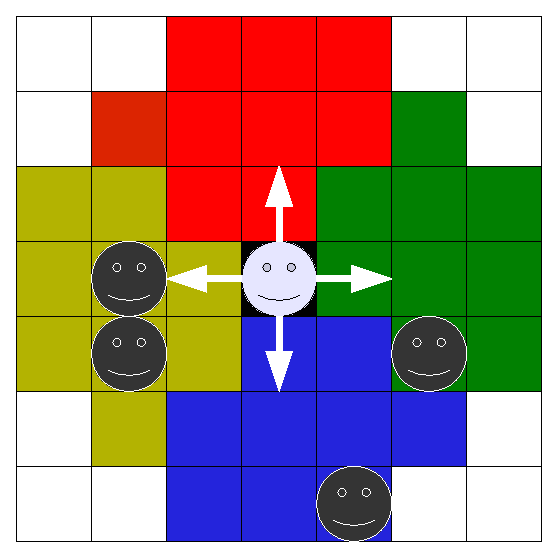
\includegraphics{agent_random.eps}
}
\caption[Caption as shown in list of figures]{Agent bewegt sich in eine zuf\"allige Richtung (oder bleibt stehen)}
\label{agent_random:fig}
\end{figure}

\subsection{``Simple AI Agent''}
Ist der Zielagent in Sichtweite, bewegt sich dieser Agent auf das Ziel zu. Ist das Ziel nicht in Sichtweite, f\"uhrt er eine zuf\"allige Aktion aus.

\begin{figure}[htbp]
\centerline{	
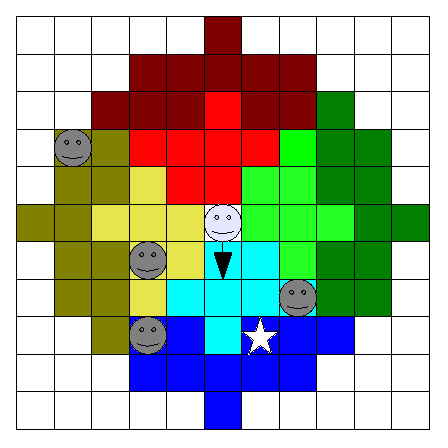
\includegraphics{simple_agent_to_goal.eps}
}
\caption[Caption as shown in list of figures]{Agent bewegt sich auf Zielagent zu (sofern sichtbar)}
\label{simple_agent_to_goal:fig}
\end{figure}

\subsection{``Intelligent AI Agent''}
Ist der Zielagent in Sicht, verh\"alt sich dieser Algorithmus wie ``Simple AI Agent''. Ist der Zielagent dagegen nicht in Sicht, wird versucht anderen Agenten auszuweichen um ein m\"oglichst breit gestreutes Netz aus Agenten aufzubauen. In der Implementation hei\ss{}t das, dass unter allen Richtungen, in denen kein anderer Agent geortet wurde, eine zuf\"allig ausgew\"ahlt wird. Falls alle Richtungen belegt (oder alle frei) sind, aus allen Richtungen eine zuf\"allig ausgew\"ahlt wird.

\begin{figure}[htbp]
\centerline{	
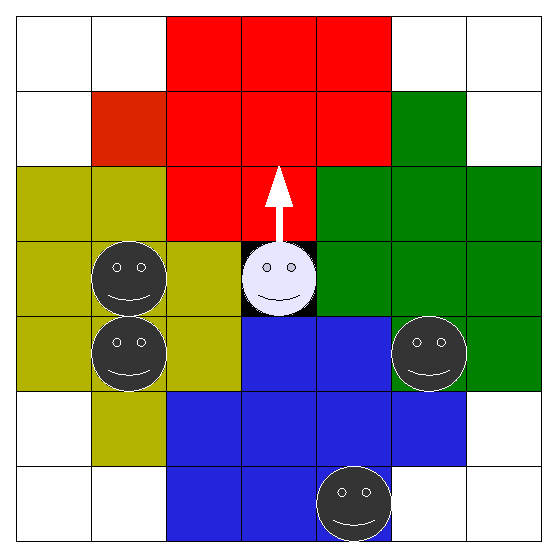
\includegraphics{intelligent_agent.eps}
}
\caption[Caption as shown in list of figures]{Agent bewegt sich von anderen Agenten weg (falls Zielagent nicht sichtbar)}
\label{intelligent_agent:fig}
\end{figure}

\section{Grunds\"atzliche Zielagententypen}

Die Art der Bewegung des Zielagenten tr\"agt grunds\"atzlich zur Schwierigkeit eines Szenarios bei. Gemeinsam haben alle Arten von Bewegungen des Zielagenten, dass, wenn kein freies Feld zur Verf\"ugung steht, springt der Zielagent auf ein zuf\"alliges freies Feld auf dem Grid springt. Dies kommt einem Neustart gleich und ist notwendig um einer Verf\"alschung des Ergebnisses zu verhindern, das dadurch r\"uhren kann, dass ein oder mehrere Agenten (zusammen mit eventuellen Hindernissen) bis zum Ende des Problems alle vier Bewegungsrichtungen des Zielagenten blockieren.


\subsection{``Random Movement''}
Wie ``Randomized''. Sind alle m\"oglichen Felder belegt, wird wie oben beschrieben auf ein zuf\"alliges Feld gesprungen.

\subsection{``Total Random''}
Der Zielagent springt zu einem zuf\"alligen (freien) Feld auf dem Grid. Mit dieser Einstellung kann die Abdeckung des Algorithmus gepr\"uft werden, d.h. inwieweit die Agenten jeweils au\ss{}erhalb der \"Uberwachungsreichweite anderer Agenten bleiben. Jegliche Anpassung an die Bewegung des Zielagenten ist hier wenig hilfreich, ein Agent kann nicht einmal davon ausgehen, dass sich der Zielagent in der N\"ahe seiner Position der letzten Zeiteinheit befindet.

\subsection{``One direction change''}
Mit dieser Einstellung wird die der letzten Richtung entgegengesetzten Richtung aus der Menge der Auswahlm\"oglichkeiten entfernt und von den verbleibenden drei Richtungen (plus der Aktion ``Stehenbleiben'') eine zuf\"allig ausgew\"ahlt. Sind alle drei Richtungen versperrt, wird stehengeblieben.
War die letzte Aktion nicht eine Bewegungsrichtung sondern die Aktion ``Stehenbleiben'', so wird eine zuf\"allige Richtung ausgew\"ahlt. Sind alle Richtungen versperrt wird auch hier wie bei ``Random Movement'' auf ein zuf\"alliges Feld gesprungen.

\begin{figure}[htbp]
\centerline{	
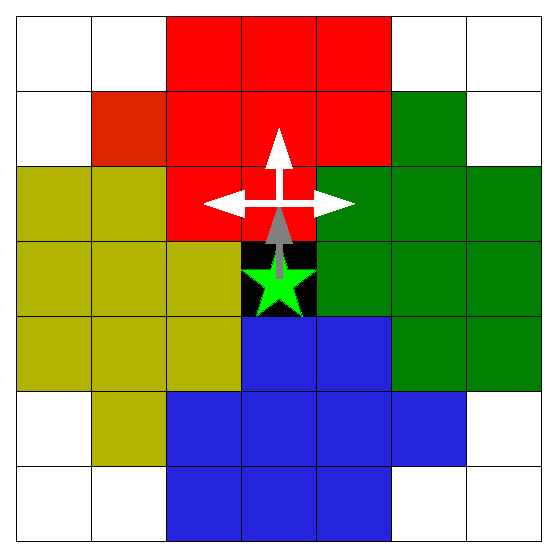
\includegraphics{goal_direction_change.eps}
}
\caption[Caption as shown in list of figures]{Zielagent macht pro Schritt maximal eine Richtungs\"anderung}
\label{goal_agent_one_direction_change:fig}
\end{figure}

\subsection{``Always same direction''}
Der Zielagent versucht immer Richtung Norden zu gehen. Ist das Zielfeld blockiert, w\"ahlt er ein zuf\"alliges, angrenzendes, freies Feld im Westen oder Osten. Sind auch diese belegt, springt er wie oben auf ein zuf\"alliges freies Feld. Schafft es der Zielagent innerhalb von einer bestimmten Zahl (Breite des Spielfelds) von Schritten nicht, einen weiteren Schritt nach Norden zu gehen, wird ebenfalls gesprungen um ein Festh\"angen an einem Hindernis zu vermeiden.

\begin{figure}[htbp]
\centerline{	
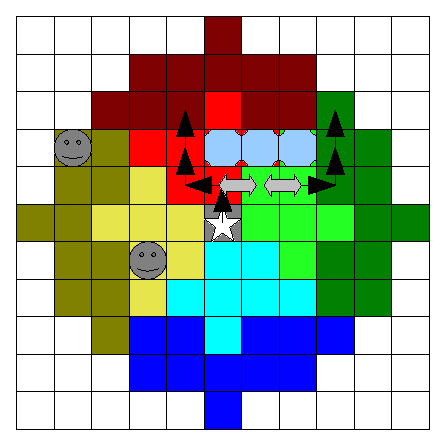
\includegraphics{goal_always_same_direction.eps}
}
\caption[Caption as shown in list of figures]{Zielagent bewegt sich, wenn m\"oglich, immer nach Norden}
\label{goal_agent_always_same_direction:fig}
\end{figure}

\subsection{``Intelligent (Open)''}
Der Zielagent versucht andere Agenten zu vermeiden. Bei der Wahl der Richtung werden alle Richtungen gestrichen, in denen sich ein anderer Agent befindet. Von den verbleibenden Richtungen werden mit 20\% Wahrscheinlichkeit alle Richtungen gestrichen, in denen sich ein Hindernis befindet. Sind alle Richtungen gestrichen worden, bewegt der Zielagent sich zuf\"allig. Sind alle Richtungen blockiert, springt er wie in den anderen Einstellungen auch.

\begin{figure}[htbp]
\centerline{	
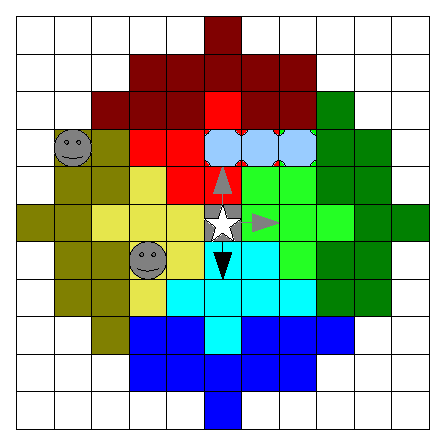
\includegraphics{goal_intelligent_open.eps}
}
\caption[Caption as shown in list of figures]{Zielagent bewegt sich von Agenten und mit bestimmter Wahrscheinlichkeit von Hindernissen weg}
\label{goal_agent_intelligent_open:fig}
\end{figure}

\subsection{``Intelligent (Hide)''}
Der Zielagent vermeidet andere Agenten wie bei ``Intelligent (Open)'', streicht aber statt Richtungen mit Hindernissen Richtungen ohne Hindernisse mit 20\% Wahrscheinlichkeit.

\begin{figure}[htbp]
\centerline{	
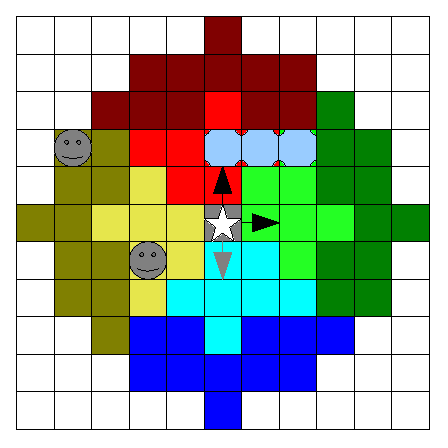
\includegraphics[width=0.45\columnwidth]{goal_intelligent_hide.eps}
}
\caption[Caption as shown in list of figures]{Zielagent bewegt sich von Agenten weg und mit bestimmter Wahrscheinlichkeit auf Hindernissen zu}
\label{goal_agent_intelligent_hide:fig}
\end{figure}

\subsection{``LCS''}
Eine LCS Implementierung die der der Implementierung eines LCS Agenten entspricht. Das Ziel des Zielagenten ist es hier aber, m\"oglichst nicht andere Agenten zu \"uberwachen (bzw. umgekehrt sich von anderen nicht \"uberwachen zu lassen, d.h. nicht in die \"Uberwachungsreichweite anderer Agenten zu geraten). Eine genaue Beschreibung folgt weiter unten.


\chapter{Szenarien}

Getestet werden eine Reihe von Szenarien (in Verbindung mit unterschiedlichen Werte f\"ur die Anzahl der Agenten, Gr\"o\ss{}e des Spielfelds und Art und Geschwindigkeit der Zielagentenbewegung). Wesentliche Rolle spielt hier die Verteilung der Hindernisse.
In den Darstellungen repr\"asentieren rote Felder Hindernisse, weisse Felder Agenten und das gr\"une Feld jeweils den Zielagenten.

\begin{wrapfigure}{r}{0.5\textwidth}
  \begin{center}
    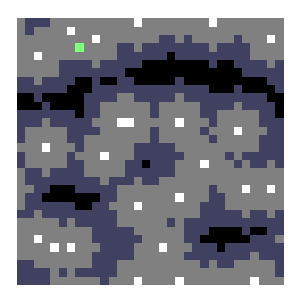
\includegraphics{00_000_grid.eps}
  \end{center}
  \caption{``Leeres Szenario''}
\end{wrapfigure}

\section{Zuf\"alliges Szenario}
Zwei Parameter bestimmen, wie das zuf\"allige Szenario auszusehen hat, zum einen der Prozentsatz an Hindernissen an der Gesamtzahl der Felder, zum anderen der Grad  inwieweit die Hindernisse zusammenh\"angen. Dieser Grad bestimmt nach Setzen eines Hindernisses die Wahrscheinlichkeit f\"ur jedes einzelne angrenzende freie Feld, dass dort sofort ein weiteres Hindernis gesetzt wird. Ein Wert von \(0.0\) ergibt somit ein v\"ollig zuf\"allig verteilte Menge an Hindernissen w\"ahrend ein Wert nahe eine oder mehrere stark zusammenh\"angende Strukturen schafft.
Wird der Prozentsatz an Hindernissen auf Null gesetzt, dann werden Hindernisse vollst\"andig deaktiviert. Als Optimierung werden in diesem Fall auch alle Sensorinformationen diesbez\"uglich deaktiviert. TODO optional


\section{Pillar Scenario}
Hier werden mit jeweils 7 Feldern Zwischenraum zwischen den Hindernissen (und mindestens 3 Feldern Zwischenraum zwischen Rand und den Hindernissen) Hindernisse verteilt. Idee ist, dass die Agenten eine kleine Orientierungshilfe besitzen aber gleichzeitig m\"oglichst wenig Hindernisse verteilt werden. TODO
Der Zielagent startet in der Mitte.


\begin{wrapfigure}{r}{0.5\textwidth}
  \begin{center}
    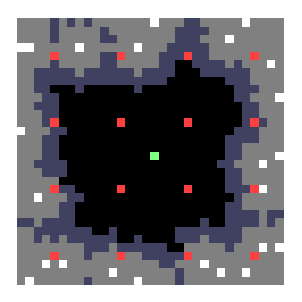
\includegraphics{pillar_grid.eps}
  \end{center}
  \caption{``S\"aulen Szenario'' : Regelm\"a\ss{}ig angeordnete Hindernisse}
\end{wrapfigure}

\begin{figure}[htbp]
\centerline{	
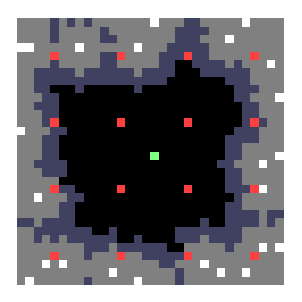
\includegraphics{pillar_grid.eps}
}
\caption[``S\"aulen Szenario'']{``S\"aulen Szenario'' : Regelm\"a\ss{}ig angeordnete Hindernisse (rot), zuf\"allige Verteilung von Agenten am Rand (weiss) und feste Startposition des Zielagenten in der Mitte (gr\"un)}
\label{pillar_grid:fig}
\end{figure}

\section{Cross Scenario}
Hier gibt es in der Mitte eine horizontale Reihe aus Hindernissen halber Gesamtbreite welche durch eine vertikale Reihe aus Hindernissen halber Gesamth\"ohe geschnitten wird.

\begin{figure}[htbp]
\centerline{	
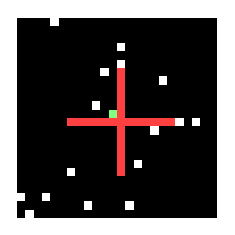
\includegraphics{cross_grid.eps}
}
\caption[Caption as shown in list of figures]{``Cross scenario'' : Zentrierte, kreuzf\"ormige Anordnung der Hindernisse (rot), zuf\"allige Verteilung der Agenten (weiss) und dem Zielagenten (gr\"un) mit fester Startposition in der Mitte}
\label{cross_grid:fig}
\end{figure}

\section{Room scenario}
In der Mitte des Grids wird ein Rechteck der halben Gesamth\"ohe und -breite des Grids erstellt, welches eine \"Offnung von 4 Feldern Breite aufweist. Der Zielagent startet wie im Pillar Scenario in der Mitte, alle Agenten starten am Rand des Grids.

\begin{figure}[htbp]
\centerline{	
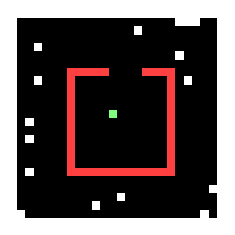
\includegraphics{room_grid.eps}
}
\caption[Caption as shown in list of figures]{``Room Scenario'' : Zentrierte, quaderf\"ormige Anordnung der Hindernisse (rot) mit \"Offnung oben, zuf\"allige Verteilung der Agenten (weiss) am Rand und der Zielagenten (gr\"un) mit festem Startpunkt in der Mitte}
\label{room_grid:fig}
\end{figure}


\section{Difficult Scenario}
Hier wird das Grid zum einen an der rechten Seite vollst\"andig durch Hindernisse blockiert um den Torus zu halbieren. Alle Agenten starten am linken Rand, der Zielagent startet auf der rechten Seite.
In regelm\"a\ss{}igen Abst\"anden (7 Felder Zwischenraum) befindet sich eine vertikale Reihe von Hindernissen mit \"Offnungen von 4 Feldern Breite abwechselnd im oberen Viertel und dem unteren Viertel.

\begin{figure}[htbp]
\centerline{	
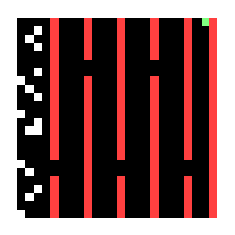
\includegraphics{difficult_grid.eps}
}
\caption[Caption as shown in list of figures]{``Difficult Scenario'' : Feste, wandartige Verteilung von Hindernissen (rot) in regelm\"a\ss{}igen Abst\"anden mit \"Offnungen, Agenten (weiss) mit zuf\"alligem Startpunkt am linken Rand und dem Zielagenten (gr\"un) mit festem Startpunkt rechts oben}
\label{difficult_grid:fig}
\end{figure}

\section{Maze Scenario}

TODO

\begin{figure}[htbp]
\centerline{	
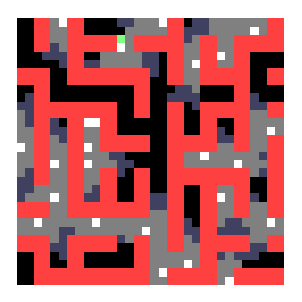
\includegraphics{maze_grid.eps}
}
\caption[Caption as shown in list of figures]{``Maze Scenario'' : TODO}
\label{maze_grid:fig}
\end{figure}

\chapter{Ablauf der Simulation}

Bei Simulationen am Computer stellt sich sofort die Frage nach der Genauigkeit. Die Agenten werden bei dieser Simulation nacheinander abgearbeitet und bewegen sich auf einem diskreten Grid. Dies kann u.U. dazu f\"uhren, dass je nach Position in der Liste abzuarbeitender Agenten die Informationen \"uber die Umgebung unterschiedlich alt sind. Die gro\ss{}e Frage ist deshalb, in welcher Reihenfolge Sensordaten ermittelt, ausgewertet, Agenten bewegt, intern sich selbst bewertet und global die Qualit\"at gemessen wird.
Einzige Restriktionen sind, dass eine Aktion nach der Verarbeitung der Sensordaten stattfinden muss und eine Bewertung einer Aktion nach dessen Ausf\"uhrung stattfinden muss. Ansonsten gibt es folgende M\"oglichkeiten:

\section{Reihenfolge der Ausf\"uhrung}
\begin{enumerate}
\item F\"ur alle Agenten werden erst einmal die neuen Sensordaten erfasst und sich f\"ur eine Aktion entschieden. Sind alle Agenten abgearbeitet werden die Aktionen ausgef\"uhrt.
\item Die Agenten werden nacheinander abgearbeitet, es werden jeweils neue Sensordaten erfasst und sich sofort f\"ur eine neue Aktion entschieden. 
\end{enumerate}

Bei der ersten M\"oglichkeit haben alle Agenten die Sensordaten vom Beginn der Zeiteinheit, w\"ahrend bei der zweiten M\"oglichkeit sp\"ater verarbeitetere Agenten bereits die Aktionen der bereits berechneten Agenten miteinbeziehen k\"onnen. Umgekehrt k\"onnen dann fr\"uhere Agenten bessere Positionen fr\"uher besetzen. Da aufgrund der primitiven Sensoren nicht davon auszugehen ist, dass Agenten beginnende Bewegungen (und somit deren Zielposition) anderer Agenten einbeziehen k\"onnen, soll jeder Agent von den Sensorinformationen zu Beginn der Zeiteinheit ausgehen.
Die Reihenfolge der Ausf\"uhrung der Aktionen spielt eine Rolle, wenn mehrere Agenten sich auf das selbe Feld bewegen wollen. Arbeiten wir die Liste unserer Agenten einfach linear ab, haben vorne stehende Agenten eine h\"ohere Wahrscheinlichkeit, dass ihre Aktion ausgef\"uhrt wird. Da es keine Veranlassung gibt, ihnen diesen Vorteil zu geben, werden Aktionen in zuf\"alliger Reihenfolge abgearbeitet. Bez\"uglich der Bewegung ergibt sich hierbei eine weitere Frage, n\"amlich wie unterschiedliche Bewegungsgeschwindigkeiten behandelt werden sollen. Alle Agenten haben eine Einheitsgeschwindigkeit von maximal einem Feld pro Zeiteinheit, w\"ahrend sich der Zielagent je nach Szenario gleich eine ganze Anzahl von Feldern bewegen kann. Auch hier habe ich mich f\"ur eine zuf\"allige Verteilung entschieden. Kann sich der Zielagent um n Schritte bewegen, so wird seine Bewegung in \(n\) Einzelschritte unterteilt, die nacheinander mit zuf\"alligen Abst\"anden (d.h. Bewegungen anderer Agenten) ausgef\"uhrt werden.
Eine weitere Frage ist, wie der Zielagent diese weiteren Schritte festlegen soll. Hier soll ein Sonderfall eingef\"uhrt, so dass der Zielagent in einer Zeiteinheit mehrmals (\(n\)-mal) neue Sensordaten erfassen und sich f\"ur eine neue Aktion entscheiden kann.

\section{Reihenfolge Rewardverteilung}
Schlie\ss{}lich bleibt die Frage danach, wann gepr\"uft werden soll, ob der Zielagent in Sicht ist, und wann somit der Reward verteilt wird. Da XCS in der Standardimplementation darauf ausgelegt ist, den Reward jeweils genau einer Aktion zuzuordnen, sollte der Reward nicht bei jeder einzelnen Bewegung des Zielagenten \"uberpr\"uft und verteilt werden, sondern nur einmal pro Zeiteinheit. Au\ss{}erdem soll der Einfachheit halber der Reward auch von bin\"arer Natur sein (�Zielagent in \"uberwachungsreichweite� oder �Zielagent nicht in \"uberwachungsreichweite�), weshalb Zwischenzust\"ande f\"ur den Reward (z.B. �War zwei von drei Zeitschritten in der \"uberwachungsreichweite� => 2/3 Reward) ausgeschlossen werden sollen. F\"ur den Reward gibt es somit folgende M\"oglichkeiten:

\begin{enumerate}
\item Rewards werden direkt nach der Ausf\"uhrung einer einzelnen Aktion vergeben
\item Rewards werden nach Ausf\"uhrung aller Aktionen der Agenten vergeben
\item Rewards werden nach Ausf\"uhrung aller Aktionen des Zielagenten vergeben
\end{enumerate}

Werden die Rewards sofort vergeben (Punkt 1), dann werden sich sp\"ater noch weg-bewegende bzw. sich sp\"ater noch hin-bewegende Agenten nicht beachtet. Da die Agenten in zuf\"alliger Reihenfolge abgearbeitet werden, w\"urde das bedeuten, dass die Bewegung der restlichen (zuf\"alligen) Anzahl von Agenten in den Reward nicht miteinbezogen wird. Selbiges gilt f\"ur Punkt 3. 
Auch der Zielagent kann Reward erhalten. Hierbei gibt es ebenfalls drei M\"oglichkeiten:
\begin{enumerate}
\item Reward direkt nach Ausf\"uhrung des letzten Schritts
\item Reward nach Ausf\"uhrung aller Agenten
\end{enumerate}

Eine konkrete Antwort kann man auf diese zwei Fragen nicht geben, sie h\"angt n\"amlich davon ab, was man denn nun eigentlich erreichen m\"ochte, also auf welche Weise die Qualit\"at des Algorithmus bewertet wird. Der naheliegendste Messzeitpunkt ist nachdem sich alle Agenten bewegt haben. Da wir Agenten und Zielagenten in einem Durchlauf gemeinsam bewegen, stellt sich die Frage nicht, ob wir wom\"oglich vor der Bewegung des Zielagenten die Qualit\"at messen sollen. Eine Messung nach der Bewegung des Zielagenten w\"urde diesem erlauben, sich vor jeder Messung optimal zu positionieren, was in einer geringeren Qualit\"at f\"ur den Algorithmus resultiert, da sich der Zielagent aus der \"Uberwachungsreichweite anderer Agenten hinausbewegen kann. Letztlich ist es eine Frage der Problemstellung, denn eine Messung nach Bewegung des Zielagenten bedeutet letztlich, dass ein Agent, einen gerade aus seiner \"Uberwachungsreichweite heraus laufenden Zielagenten in diesem Schritt nicht mehr \"uberwachen kann.
Da ein wesentlicher Bestandteil die Kooperation (und somit die Abdeckung des Spielfelds anstatt dem Verfolgen des Zielagenten) sein soll, soll ein Bewertungskriterium sein, inwieweit der Einfluss des Zielagenten minimiert werden soll. Auch findet, wenn wir vom realistischen Fall ausgehen, die Bewegung des Zielagenten gleichzeitig mit allen anderen Agenten statt. Die Qualit\"at wird somit nach der Bewegung des Zielagenten gemessen. Die \"Uberlegung unterstreicht auch nochmal, dass es besser ist, den Zielagenten insgesamt wie einen normalen (aber sich mehrmals bewegenden) Agenten zu behandeln.
Was den Zeitpunkt des Rewards betrifft, lautet die Hypothese, dass wir ein besseres Ergebnis erreichen, wenn man den Reward anhand der selben Momentaufnahme verteilt, anhand der wir auch die Qualit\"at testen, d.h. dass Punkt 2 Punkt 1 \"uberlegen ist. Dies best\"atigt sich in Tests siehe TODO.

\section{Zusammenfassung}
Zusammenfassend sieht der Ablauf aller Agenten (inklusive des Zielagenten) also wie folgt aus:

\begin{figure}[H]
\setbox0\vbox{\small
\begin{enumerate}
\item Erfassung aller Sensordaten
\item Wahl der Aktion anhand der Regeln des jeweiligen Agenten
\item Ausf\"uhrung der Aktion (in zuf\"alliger Reihenfolge, der Zielagent f\"uhrt nach dem ersten Schritt au\ss{}erdem Schritt 1. und 2. f\"ur alle weiteren Schritte nochmals durch)
\item Bestimmung des Rewards
\item Bestimmen der Qualit\"at dieser Zeiteinheit
\end{enumerate}
}
\centerline{\fbox{\box0}}
\end{figure}

\chapter{Erste Analyse der Agenten ohne LCS}

In diesem Kapitel sollen erste Analysen bez\"uglich der verwendeten Szenarien anhand des zuf\"alligen Algorithmus, des Algorithmus mit einfacher Intelligenz (``Simple AI Agent'') und des Algorithmus mit komplexerer Regeln (``Intelligent AI agent'') angefertigt werden. Die Ergebnisse aus der Analyse werden eine Grundlage f\"ur die vergleichende Betrachtung der Agenten mit LCS Algorithmen dienen.

\section{Total Random Goal Agent Movement}

In allen Szenarien mit dieser Form der Bewegung des Zielagenten kommt es nur darauf an, dass die Agenten einen m\"oglichst gro\ss{}en Bereich des Grids abdecken. In allen Standardszenarios zeigt sich, dass der ``Simple AI Agent'' sich wie erwartet nicht wesentlich vom zuf\"alligen Agenten unterscheidet. 

\subsection{Ohne Hindernisse}

Ohne Hindernisse gibt sich ein klares Bild. Das Ergebnis der einfachen KI ist etwas schlechter als der des zuf\"alligen Agenten, da sich immer wenn mehrere Agenten den Zielagenten in der selben Richtung in Sichtweite haben, sich mehrere Agenten in die selbe Richtung bewegen. Dies beeintr\"achtigt die zuf\"allige Verteilung der Agenten auf dem Spielfeld und f\"uhrt somit auch zu einer niedrigeren Abdeckung des Grids.
Der intelligente Agent liegt hier sehr deutlich vorne, ein m\"oglichst weitr\"aumiges Verteilen auf dem Feld f\"uhrt zum Erfolg, denn genau das wird mit dem v\"ollig zuf\"allig springenden Agenten getestet.

\subsection{Zuf\"allig verteilte Hindernisse}

Hier ergeben sich bei allen Einstellungen des ``Connection Factors'' und ''Obstacle Factors'' ebenfalls ein klares Bild, der intelligente Agent liegt wieder vorne, dann kommt allerdings schon der einfache Agent mit bis zu 10\% zum zuf\"alligen Agenten. Der wesentliche zweite Faktor ist hier, dass der einfache Agent, wenn er den Zielagenten in Sicht hat, davon ausgehen kann, dass sich in dieser Richtung wahrscheinlich kein Hinderniss befindet, w\"ahrend der zuf\"allige Agent Hindernisse \"uberhaupt nicht beachtet, somit \"ofters gegen ein Hinderniss l\"auft und letztlich \"ofters stehen bleibt. Der Unterschied zwischen beiden Agenten ist besonders hoch in Szenarien mit gr\"o\ss{}erem Anteil an Hindernissen.
Ansonsten liegt der intelligente Agent wieder eindeutig vorne, beherrscht aber besonders gut Szenarien hohem ``Connection Factor'' (\(1.0\)) der geringem Anteil an Hindernissen (\(0.1\)), bei denen er bis zu etwa 15\% \"uber dem Ergebnis des einfachen Agenten liegt.
Dies liegt daran, dass Szenarien mit hohem ``Connection Factor'' bedeuten, dass alle Hindernisse zusammenh\"angend einen gro\ss{}en Block bilden und somit dem Szenario ohne Hindernissen \"ahnlich sind, auf dem dieser Agent ja besonders gut abschneidet. In zerkl\"uftete Szenarien hat der Algorithmus dagegen Schwierigkeiten um andere Agenten \"uberhaupt zu Gesicht bekommen, der Vorteil der Verteilung f\"allt also zu einem Teil weg. 

Dies best\"atigt auch ein Durchlauf bei dem Sichtbehinderungen durch Hindernisse deaktiviert sind. Hierbei erreicht der intelligente Agent im Szenario (\(0.4\), \(0.1\)) statt TODO evtl weg

\section{Random Neighbor und One Direction Change}

Wesentlicher Punkt bei beiden Szenarien ist, dass der jetzige Ort des Zielagenten maximal zwei Felder (die Standardgeschwindigkeit des Zielagenten in den Tests) vom Ort in der vorangegangenen Zeiteinheit entfernt ist. Somit ist ein lokales Einfangen eher von Relevanz, wenn auch der Zielagent grunds\"atzlich schneller als andere Agenten ist.

Dementsprechend ist der einfache Agent bei einem Hinderniss-Anteil von \(0.0\) bis \(0.1\) besser als alle anderen Agenten und dementsprechend ist bei allen Tests der zuf\"allige Agent weit abgeschlagen.
Ab einem Anteil von \(0.2\) liegt jedoch der intelligente Agent vorne. Dies liegt schlicht an der Zahl der Agenten relativ zur hindernissfreien Fl\"ache, da sich die Agenten in m\"oglichst gro\ss{}em Abstand zueinander positionieren.

Im Falle des ``One Direction Change'' bewegt sich der Agent im Grunde nur etwas schneller, da er es vermeidet, auf das urspr\"ungliche Feld zur\"uckzukehren.
TODO? Vielleicht sogar Random Neighbor raus...

\section{Intelligent Open}

\section{Intelligent Hide}

TODO:Beide gleiche Ergebnisse?Source pr\"ufen


\section{Always Same Direction}

TODO

\section{LCS}

Wird weiter unten besprochen.





\section{Zusammenfassung}

Wie wir gesehen haben gibt es also Szenarien in denen Abdeckung kaum eine Rolle spielt und lokale Entscheidungen eine wesentliche Rolle spielen. Dies wird es erleichtern, geeignete Szenarien im Kapitel ``Kommunikation'' zu finden.




TODO Anpassung LCS an unterschiedliche Sichtreichweiten?



\chapter{LCS}

\section{Einf\"uhrung}

Jeder Agent besitzt ein Learning Classifier System, welches auf dem von Butz TODO XCS basiert. Die Implementierung entspricht im Wesentlichen der Standardimplementation von Butz 2000, eine Besonderheit stellt allerdings die Problemdefinition dar. Keine der gegenw\"artigen Implementationen und Varianten von XCS besch\"aftigen sich mit dynamischen \"Uberwachungsszenarios sondern mit Szenarios, bei denen das Ziel in einer statischen Umgebung gefunden werden muss. 

Im XCS-Multistepverfahren (TODOLiteratur) l\"auft ein Problem so lange bis ein positiver Reward aufgetreten ist und startet dann das Szenario neu. Bei einem \"Uberwachungsszenario mit kontinuierlichem Reward ist das Multistepverfahren nicht anwendbar, das Szenario kann nicht neugestartet werden, da sich die Agenten w\"ahrend des Laufs anpassen sollen. Ziel ist hier ja nicht, einen bestimmten Weg zu einem festen Ziel zu finden (wie z.B. bei WOODS TODO), sondern eine bestimmte Regelmenge zu erlernen, mit der eine m\"oglichst gute, dauerhafte \"Uberwachung stattfinden kann. 

In der hier verwendeten Implementierung l\"auft das Problem deshalb einfach weiter. Wesentlicher Unterschied zu XCS wird deshalb die Behandlung des Rewards sein.

In der Literatur fehlen Arbeiten, in denen ein solches Szenario (ohne globale Steuerungseinheit oder Regeltausch) in Verbindung mit dem XCS behandelt wird. Diese Arbeit soll diese L\"ucke schlie\ss{}en und die Basis f\"ur weitere Arbeiten in dieser Richtung liefern.


TODO anfaengliche Initialisierung?

\section{Classifier}

Ein LCS beinhaltet eine Reihe von Classifiern. Ein einzelner Classifier besteht im Wesentlichen aus f\"unf Teilen:

\subsection{Fitness}
Der Fitness Wert soll die allgemeine Genauigkeit des Classifiers 
repr\"asentieren und wird \"uber die Zeit hinweg sukzessive an die beobachteten Rewards angepasst. TODO Wilson. Der Wertebereich verl\"auft zwischen \(0.0\) und \(1.0\) (maximale Genauigkeit).

\subsection{Prediction}
Der ``Prediction''-Wert des Classifiers stellt die H\"ohe des Rewards dar, von dem der Classifier vermutet, dass er ihn bei der n\"achsten Vergabe des Rewards erhalten wird. Auch dieser Wert wird stetig angepasst.

\subsection{Prediction Error}
Der �Prediction-Error�-Wert soll die Genauigkeit des Classifiers bzgl. der Reward-Prediction (durchschnittliche Differenz zwischen Prediction und tats\"achlichem Reward) repr\"asentieren. U.a. auf Basis dieses Werts wird der Fitness-Wert des Classifiers angepasst.

\subsection{Aktion}
Wird ein Classifier ausgew\"ahlt, wird eine bestimmte Aktion ausgef\"uhrt. In unserem Szenario entsprechen die Aktionsm\"oglichkeiten die der anderen Agenten, also 4 Bewegungsrichtungen plus eine ``nichts-tun''-Aktion.

\subsection{Kondition}
Die Kondition gibt an, bei welchem Sensor-Input dieser Classifier ausgew\"ahlt werden kann. 

\section{Sensoren und Matching}

In der hier verwendeten Implementierung gibt es zwar eine gewisse Vorverarbeitung der Sensordaten, im Wesentlichen m\"ussen aber Kondition und Sensordaten \"ubereinstimmen, damit der jeweilige Classifier ausgew\"ahlt wird. Konkret besteht die Kondition ebenfalls aus einem 9-stelligen Vektor, der allerdings nicht nur bin\"are sondern trin\"are Werte besitzen kann. 

\subsection{Wildcards}

Neben den zu den Sensordaten korrespondierenden Werten 0 und 1 gibt es noch einen dritten ``dont-care''-Zustand ``\#'', der anzeigen soll, dass beim Vergleich zwischen Kondition und Sensordaten diese Stelle ignoriert werden soll. Eine aus nur ``dont-care'' Werten bestehende Kondition w\"urde somit bei der Auswahl immer in Betracht gezogen werden, da er auf alle Sensor-Inputs passt.

Beispiel:
Kondition \(1.\#010.1\#01\) matched Sensordaten \(1.0010.1001\), \(1.1010.1001\), \(1.0010.1101\) und \(1.1010.1101\).

Die Benutzung von Wildcards erlaubt es dem LCS mehrere Classifier zu subsummieren, wodurch die Gesamtzahl der Classifier sinkt und somit Erfahrungen, die ein LCS Agent sammelt, nicht unbedingt doppelt gemacht werden m\"ussen. Die dahinter stehende Annahme ist, dass es Situationen gibt, in denen ein Wert aus dem Sensor-Input f\"ur die Qualit\"at der Entscheidung weniger entscheidend sein kann, als die Ersparnis durch das Zusammenlegen beider Classifier, d.h. dem Ignorieren dieses Inputs.

\subsection{Matching von Sensordaten mit Classifiern}

Beim Vergleich mit Sensordaten wir ebenfalls mit einem Vektor wie bei \(B\) erglichen. Entscheidend beim Vergleich ist hier aber nicht, dass beide Vektoren identisch sind, sondern, dass der Classifier ``matched''. Ein Element des Bedingungsvektors kann 3 Zust\"ande einnehmen. \(0\), \(1\) und \(\#\). \(\#\) beinhaltet beide Zust\"ande \(0\) und \(1\).

Den dritten verwendeten Vergleich zwischen Bedingungsvektoren gibt es bei der Subsumation (der Kinder zu ihren Eltern und des gesamten ActionSets siehe ~(\ref{sec:subsummation}). Ein Classifier subsumiert einen anderen Classifier, wenn er ihn beinhaltet, aber nicht identisch mit ihm ist, also allgemeiner ist.

\subsection{Drehungen}

Ein Classifier besteht aus dem Bedingungsvektor \[(g x_{0} x_{1} x_{2} x_{3})\] (bzw. \[(g x_{0} x_{1} x_{2} x_{3} y_{0} y_{1} y_{2} y_{3})\] f\"ur den Fall mit Hindernissen) und der Aktion \(a\).

Eine wesentliche Vereinfachung, die angenommen wird, ist, dass angenommen wird, dass eine Aktion in einer anderen, in 90 Grad Schritten gedrehten Umwelt, gleiche G\"ute besitzt.
In einer statischen Umgebung ist dies nicht unbedingt der Fall, ohne diese Vereinfachung k\"onnte sich ein Agent einfacher zurechtfinden, wie TODO (keine Drehung, 1 Problem pro Experiment) diese Testl\"aufe zeigen.
Da wir uns aber auf den dynamischen Fall konzentrieren und durch diese Vereinfachung eine signifikante Verkleinerung des Suchraums erreichen, benutzen wir die Vereinfachung.
Im Algorithmus betrifft dies prim\"ar den Vergleich von Classifiern untereinander und mit dem Sensorstatus. 

\subsection{\"Aquivalenz von Classifiern}
Ein Classifier A ist identisch mit einem Classifier B wenn gilt:

\begin{enumerate}
\item \[A_{g} = B_{g}\]
\item Falls \[A_{g} = 0\]:

\begin{enumerate}
\item Es gibt ein \(i\) f\"ur das gilt: \[(A_{x_{0+i \bmod 4}} A_{x_{1+i \bmod 4}} A_{x_{2+i \bmod 4}} A_{x_{3+i \bmod 4}}) = (B_{x_{0}} B_{x_{1}} B_{x_{2}} B_{x_{3}})\]
\item Mit Hindernissen muss f\"ur dieses \(i\) au\ss{}erdem gelten: 

\begin{enumerate}
\item \[(A_{y_{0+i \bmod 4}} A_{y_{1+i \bmod 4}} A_{y_{2+i \bmod 4}} A_{y_{3+i \bmod 4}}) = (B_{y_{0}} B_{y_{1}} B_{y_{2}} B_{y_{3}}\]
\item Falls \(A_{a} = \mathrm{NO_ACTION}\): \[A_{a} = B_{a}\]
\item Falls \(A_{a} \neq \mathrm{NO_ACTION}\): \[(A_{a}+i) \bmod 4 = B_{a}\]
\end{enumerate}
\end{enumerate}

\item Falls \(A_{g} = 1\):

\begin{enumerate}
\item \[(A_{x_{0}} A_{x_{1}} A_{x_{2}} A_{x_{3}}) = (B_{x_{0}} B_{x_{1}} B_{x_{2}} B_{x_{3}})\]
\item Mit Hindernissen muss au\ss{}erdem gelten: \[(A_{y_{0}} A_{y_{1}} A_{y_{2}} A_{y_{3}}) = (B_{y_{0}} B_{y_{1}} B_{y_{2}} B_{y_{3}})\]
\item \[A_{a} = B_{a}\]
\end{enumerate}

\end{enumerate}

Die Gleichheit zwischen Vektoren gilt, wenn paarweise Gleichheit zwischen den Elementen besteht, also \(A_{x_{i}} = B_{x_{i}}\) f\"ur \(i = 0 \dots 3\) und \(A_{y_{i}} = B_{y_{i}}\) f\"ur \(i = 0 \dots 3\) im Fall mit Hindernissen.

\subsection{Test Drehungen}

Mit aktivierter Optimierung der Drehungen wird in bestimmten Szenarien bis zu einer bestimmten Schrittzahl ein besseres Ergebnis erreicht, d.h. die Konvergenzgeschwindigkeit wird erh\"oht. In l\"angeren Durchl\"aufen mit gr\"o\ss{}erer Schrittzahl werden jedoch bessere Ergebnisse ohne der Optimierung erreicht. Der Zugewinn folgt aus einer durch die zus\"atzliche lokale Information die in den Classifiern gespeichert werden kann.

In einer zuk\"unftigen Implementierung sollte \"uberlegt werden, wie bei r\"aumlichen Aufgaben f\"ur Classifier ein LCS sowohl drehbare als auch nicht-drehbare Classifier speichern kann. Dies kann in einer Form des erw\"ahnten Wildcard-Systems bewerkstelligt werden. Dadurch und zusammen mit der Subsummation k\"onnten beide Vorteile vereint werden und sowohl lokale, als auch allgemeine Information gesammelt werden. TODOvielleicht doch noch rein?




\section{Implementation}

F\"ur die Auswahl der tats\"achlich auszuf\"uhrenden Aktion m\"ussen dann alle (genotypischen) Classifier in AppliedClassifier umgewandelt werden, die jeweils genau auf eine bestimmte Aktion verweisen.
Sichtwe

Zur Durchf\"uhrung und Forschung war es notwendig, den kompletten XCS Algorithmus nachvollziehen zu k\"onnen. TODO

Besonders die Verwaltung der Numerosity und die Verwendung des maxPrediction TODO


Das Multistepverfahren baut darauf auf, dass die Qualit\"at der Agenten sich sukzessive mit jeder Probleminstanz verbessert, der Reward eben an immer weiter vom Ziel entfernte Aktionen TODO weitergereicht wird.

Der hier entwickelte Algorithmus muss prim\"ar nicht einen Weg zum Ziel erkennen, sondern eine m\"oglichst optimale (und auch an andere Agenten angepasste) Verhaltensstrategie finden.

Da sich das Ziel schneller bewegt, kann eine einfache Verfolgungsstrategie nicht zum Erfolg f\"uhren. Eine einfache Implementation mit einem simplen Agenten der auf das Ziel zugeht, wenn es in Sicht ist und sich sonst wie ein sich zuf\"allig bewegender Agent verh\"alt, schneidet grunds\"atzlich schlechter ab.


\subsection{Numerosity}



TODO Beschreibung
In der originalen Implementierung von Butz 2000 TODO war die Behandlung der Numerosity stark optimiert auf den Fall des einmaligen Rewards ohne Protokollierung der bisherigen ActionSets. Nach einer missgl\"uckten ersten Implementierung � der Wert der numerositySum eines ClassifierSets stimmte nicht mehr mit der Summe der numerosity-Werte der enthaltenen Classifiers \"uberein � entschloss ich mich den entsprechenden Code neuzuschreiben. Hierbei wurde jedem Classifier eine Liste der Eltern, d.h. der jeweiligen ActionSets, zugewiesen.
Wird ein Microclassifier entfernt, wird dann lediglich die \"Anderungsfunktion der Numerosity des Classifiers aufgerufen, der dann wiederum die NumerositySum der jeweiligen Eltern anpasst. Dies macht einige Optimierungen r\"uckg\"angig, erspart aber sehr viel Umst\"ande, die NumerositySum immer auf den aktuellen Stand zu halten.
Positiver Nebeneffekt ist, dass man dadurch leicht auf die Menge der ActionSets zugreifen kann, denen ein Classifier angeh\"ort. Inwiefern das tats\"achlich von Nutzen sein kann ist offen. TODO
Kernst\"uck des LCS Agenten:



\subsection{Covering}

Die Implementation entspricht im Wesentlichen dem Original, es wurde aber im Hinblick auf eine klare Code-Struktur eine Optimierung entfernt und Code zur Behandlung von Drehungen hinzugef\"ugt. Im Original wird die Erstellung des MatchSets gleichzeitig mit dem Covering ausgef\"uhrt, wodurch m\"oglicherweise Zeit gespart wird, w\"ahrend in dieser Implementierung es in zwei Funktionen aufgeteilt wurde. TODOBEschreibung
Bez\"uglich der Drehung musste eine Schleife eingef\"ugt werden, die die abgedeckten Aktionen mit allen, inklusive durch Drehung entstandenen, Aktionen eines Classifiers aktualisiert. Ein einzelner Classifier kann also mehrere Aktionen abdecken, beispielsweise kann ``0-0000-0000->0'' bei der Sensoreingabe ``0-0000-0000'' alle vier Aktionen bereits abdecken. TODO besseres Beispiel. 


In meiner ersten Version hatte ich alle ung\"ultigen Aktionen von vornherein f\"ur das Covern ausgeschlossen. Eine ung\"ultige Aktion ist beispielsweise ein Laufen gegen ein Hindernis oder einen Agenten. Alleine dadurch verbesserte sich die Leistung um etwa 0.5\%. Das l\"asst sich darauf zur\"uckf\"uhren, dass die Sensoren eines Agenten eigentlich nur feststellen k\"onnen, ob ein anderer Agent in Sichtweite ist, nicht aber in welcher Entfernung. F\"ur die eigentlichen Ergebnisse wurde die daf\"ur verantwortliche Methode wieder entfernt.

Au\ss{}erdem ist ein Fehler der originalen XCS Implementation behoben. Wenn neue Classifier beim Covering hinzugef\"ugt werden, wird ihre anf\"angliche ActionSetSize auf die numerositySum des matchSets gesetzt. Einen Grund daf\"ur gibt es nicht, in meiner Implementation setze ich deshalb den Wert auf die anf\"angliche Gr\"o\ss{}e des actionSets.
Beim Aufruf des Covering-Algorithmus weiss man schon, wie gro\ss{}

TODO nein!


\subsection{Subsummation}\label{sec:subsummation}

Ein Problem ist hier nat\"urlich die Sicherstellung, dass Informationen nicht verloren gehen. Andere Arbeiten befassen sich mit der Untersuchung von der Benutzung von Wildcards. In der hier verwendeten Implementation \"ubernehme ich unver\"andert die Implementation aus der Literatur.

\subsection{Evolution\"arer Algorithmus}

Der genetische Algorithmus wurde im Wesentlichen nicht ver\"andert. Da aber die Bin\"arsensoren eng zusammenh\"angen, werden beim Crossing Over zwei feste Stellen f\"ur Crossing Over benutzt. Die Stellen trennen somit die 3 Gene, Zielagent, Agenten und feste Hindernisse.

Im Test erbrachte die Benutzung des Algorithmus wenig Unterschied.
TODO Erkl�rung


\section{Ablauf eines LCS}

\begin{enumerate}
\item Bei der Auswahl einer Aktion werden zuerst einmal alle Classifier mit denjenigen Konditionen gesucht, die auf die aktuellen Sensordaten passen. Diese bilden dann das MatchSet.
\item Im n\"achsten Schritt w\"ahlen wir einen Classifier aus diesem MatchSet aus und speichern dessen Aktion.
\item Schlie\ss{}lich bilden wir anhand des MatchSets und der gew\"ahlten Aktion das ActionSet
\end{enumerate}

\subsection{Exploration and Exploitation}

Die Auswahl in Punkt (2) kann auf verschiedene Weise erfolgen. In XCS gibt es drei M\"oglichkeiten der Auswahl, wobei man zus\"atzlich noch w\"ahrend eines Experiments zwischen den M\"oglichkeiten wechseln kann.
\begin{enumerate}
\item ``exploit'': Es wird immer ein Classifier mit dem h\"ochsten Produkt aus fitness \(*\) prediction gew\"ahlt
\item ``explore'': Es wird mit Hilfe einer Roulette-Auswahl, welche anhand des Produkts aus fitess \(*\) prediction geordnet ist, ein Classifier ausgew\"ahlt
\item ``random-explore'': Es wird ein zuf\"alliger Classifier gew\"ahlt, unabh\"angig von fitness oder prediction.
\end{enumerate}

In der XCS Implementierung sind alle drei M\"oglichkeiten zu finden, standardm\"a\ss{}ig ist jedoch M\"oglichkeit 2 zugunsten von M\"oglichkeit 3 deaktiviert.
Bei einem dynamischen \"Uberwachungsszenario ist es im Vergleich zu standardm\"a\ss{}igen statischen Szenarien weder n\"otig noch hilfreich ``random-explore'' zu nutzen. Die Idee f\"ur ``random-explore'' in einem statischen Szenario ist, dass man vermeiden m\"chte, dass das LCS immer wieder die selben Entscheidungen trifft und somit immer wieder den selben Umweltreizen ausgesetzt ist, was wiederum zu immer wieder gleichen Entscheidungen f\"uhrt usw.
Bei einem dynamischen Szenario ergibt sich das Problem nicht, andere Agenten und das Ziel sind in stetiger Bewegung und der eigene Startpunkt ist nicht fixiert. Das gewichtete ``explore'' oder gar nur ``exploit'' sollten deshalb ausreichen, wenn nicht sogar wesentlich besser abschneiden.

\subsection{Wechsel zwischen Exploration und Exploitation}

In der Standardimplementierung von XCS wird zwischen ``exploit'' und ``random-explore'' nach jedem Erreichen des Ziels umgeschalten. 

M\"oglichkeit (3.) entspricht dem Fall in der Standardimplementierung von XCS. Dabei wird bei jedem Erreichen eines positiven Rewards zwischen ``explore'' und ``exploit'' hin und hergeschaltet, was in der Standardimplementierung dem Beginn eines neuen Problems entspricht.

Hierbei gibt es mehrere verschiedene M\"oglichkeiten:

\begin{enumerate}
\item Immer ``exploit''
\item Immer ``explore''
\item Abwechselnd ``explore'' und ``exploit''
\item Zuf\"allig entweder ``explore'' oder ``exploit'' (50\% Wahrscheinlichkeit jeweils)
\item Erste H\"alfte eines jeden Problems nur ``explore'', dann nur ``exploit''
\item Wie (4.), w\"ahrend des Problems allerdings eine lineare Abnahme der Wahrscheinlichkeit von ``explore'' und eine lineare Zunahme der Wahrscheinlichkeit von ``exploit''
\item ``exploit'' wenn Ziel in Sichtweite, ``explore'' sonst
\end{enumerate}

TODO


W\"ahrend es in der 

TODO Vergleich weiter unten

\chapter{LCS Varianten}

\section{Multistepverfahren}

Als Vergleich wurde das bekannte Verfahren fast unver\"andert \"ubernommen. Wie weiter oben erw\"ahnt wird das Szenario bei einem positiven Reward aber nicht neugestartet.

Idee ist, dass der Reward, den eine Aktion (bzw. das jeweils zugeh\"orige ActionSet) erh\"alt, vom erwarteten Reward der folgenden Aktion abh\"angt. Somit wird, r\"uckf\"uhrend vom Ziel, der Reward schrittweise an vorgehende Aktionen verteilt und somit das Ziel schneller gefunden

TODO Quelle


reward = 0 ? Gebe maxPrediction des n\"achsten Zugs
reward = 1 ? Gebe maxPrediction 0, reward = 1


In jedem Schritt wird das vorherige ActionSet durch maxPrediction bzw. reward belohnt
TODO

\section{LCS Variante ohne Kommunikation}
Die Hypothese bei der Aufstellung dieser Variante des XCS-Algorithmus ist im Grunde die selbe wie beim einfachen Multistepverfahren, n\"amlich dass die Kombination mehrerer Aktionen zum Ziel f\"uhrt. Die wesentliche Verbindung beim Multistepverfahren zwischen den ActionSets der einzelnen Zeitschritte war die zeitliche N\"ahe, ein einem hoch bewerteten ActionSet folgendem ActionSet wird ebenfalls hoch bewertet.
Bei der ver\"anderten LCS Variante ist die Verbindung zwischen den ActionSets direkt die zeitliche N\"ahe zu einem Ereignis. ActionSets von jedem Schritt werden gespeichert bis ein Event auftritt und dann in Abh\"angigkeit des Alters bewertet.

\(r(a)\) bezeichnet den Reward f\"ur das ActionSet mit Alter \(a\).

$$
r(a) = \left\{ \begin{array}{rl}
  \frac{a}{\mathrm{size(ActionSet)}} &\mbox{ falls reward = $1$} \\
  \frac{1 - a}{\mathrm{size(ActionSet)}} &\mbox{ falls reward = $0$}
       \end{array} \right.
$$

bzw. bei quadratischer Rewardvergabe:

$$
r(a) = \left\{ \begin{array}{rl}
  \frac{{a}^{2}}{\mathrm{size(ActionSet)}} &\mbox{ falls reward = $1$} \\
  \frac{{1 - a}^{2}}{\mathrm{size(ActionSet)}} &\mbox{ falls reward = $0$}
       \end{array} \right.
$$


\section{Verteilung des Rewards}


Es wird auf ein Event gewartet. Ein Event ist eine \"Anderung des Rewards zwischen zwei Zeitschritten. Tritt ein solches Event auf, werden alle Aktionen seit der letzten \"Anderung absteigend belohnt bzw. bestraft.

Sonderfall:
Es tritt f\"ur einen Agenten kein Event auf.

Eine Konstante ``maxStackSize'' bestimmt, wann das Warten auf ein neues Event abgebrochen werden soll. Im Fall eines Abbruchs wird die H\"alfte des Stacks (also die \"altesten Eintr\"age) mit dem damals vergebenem Reward (welcher dem aktuellen Reward entspricht, es ist ja keine Reward\"anderung, d.h. Ein Event, eingetreten) kreditiert und vom Stack genommen. Anschlie\ss{}end wird normal weiter verfahren bis der Stack wieder voll ist bzw. bis ein Event auftritt.



\section{Events}

In XCS wird lediglich das jeweils letzte ActionSet aus dem vorherigen Zeitschritt gespeichert, in der neuen Implementierung werden dagegen eine ganze Anzahl (bis zu ``maxStackSize'') von ActionSets gespeichert. Die Speicherung erlaubt zum einen eine Verarbeitung des Rewards auf Basis einer gr\"o\ss{}eren Zahl von ActionSets und zum anderen die zeitliche Relativierung eines ActionSets zu einem Event. 
Ein Classifier wird dann jeweils r\"uckwirkend anhand des Rewards aktualisiert sobald bestimmte Bedingungen eingetreten sind.

\subsection{``Event''}\label{sec:event}

Kernst\"uck des neuen Algorithmus sind ``Events''. Im Gegensatz zur direkten Weitergabe des Rewards an die Classifier gibt es bei der Verwendung von Events eine Vorverarbeitung des Rewards anhand der vergangenen Zeitschritte. 

\begin{figure}[H]
\setbox0\vbox{\small
Ein Event tritt auf, wenn:
\begin{enumerate}
\item Positive Reward\"anderung (Zielagent war im letzten Zeitschritt nicht in \"Uberwachungsreichweite)
\item Negative Reward\"anderung (Zielagent war im letzten Zeitschritt in \"Uberwachungsreichweite)
\item \"Uberlauf des Stacks (keine Reward\"anderung in den letzten ``maxStackSize'' Schritten), Zielagent ist in \"Uberwachungsreichweite.
\item \"Uberlauf des Stacks (keine Reward\"anderung in den letzten ``maxStackSize'' Schritten), Zielagent ist nicht in \"Uberwachungsreichweite.
\end{enumerate}
}
\centerline{\fbox{\box0}}
\end{figure}


\subsection{Test der verschiedenen Exploration-Modi}

Bis auf wenige Ausnahmen (Liste) irrelevant ob man nun 50\%/50\%, absteigend o.\"a. macht.
Nur ausschlie\ss{}lich Exploration bzw. ausschlie\ss{}lich Exploitation k\"onnen gewisse Schwankungen auftreten.


Wurde die Aktion ausgew\"ahlt und sp\"ater schlie\ss{}lich ausgef\"uhrt, kommen wir nun zur Rewardvergabe. 

TODO


\subsection{Vergleich Multistep / LCS}

Szenarien, Parameter.



\chapter{LCS mit Kommunikation}

\section{L\"osungen aus der Literatur}

Da wir ein Multiagentensystem betrachten, stellt sich nat\"urlich die Frage nach der Kommunikation. In der Literatur gibt es Multiagentensysteme die auf Learning Classifier Systemen aufbauen, wie z.B. TODO Literatur. 
Alle Ans\"atze in der Literatur erlauben jedoch globale Kommunikation, z.T. Gibt es globale Classifier auf die alle Agenten zur\"uckgreifen k\"onnen, z.T. gibt es globale Steuerung. 

In dieser Arbeit betrachte ich das Szenario ohne globale Steuerung oder globale Classifier, also mit der Restriktion einer begrenzten, lokalen Kommunikation.
Geht man davon aus, dass \"uber die Zeit hinweg jeder Agent indirekt mit jedem anderen Agenten in Kontakt treten kann, Nachrichten also mit Zeitverz\"ogerung weitergeleitet werden k\"onnen, ist eine Form der globalen, wenn auch zeitverz\"ogerten, Kommunikation m\"oglich. TODO 
Eine spezielle Implementierung f\"ur diesen Fall werde ich weiter unten besprechen TODO

\section{Ablauf}

Jeder Reward, der aus einem normalen Event generiert wird, wird unter Umst\"anden an alle anderen Agenten weitergegeben. Wie ein solcher sogenannter ``externer Reward'' von diesen Agenten aufgefasst wird, h\"angt von der jeweiligen Kommunikationsvariante ab, die weiter unten besprochen werden.

Durch eine gemeinsame Schnittstelle erh\"alt jeder Agent den Reward zusammen mit dem Factor. Dabei ergibt sich das Problem, dass sich Rewards \"uberschneiden k\"onnen, da jeder Reward sich r\"uckwirkend auf die vergangenen ActionClassifierSets auswirken kann. Auch k\"onnen mehrere externe Rewards eintreffen als auch ein eigener lokaler Reward aufgetreten sein. W\"urden die Rewards nach ihrer Eingangsreihenfolge abgearbeitet, kann es passieren, dass das selbe ActionClassifierSet sowohl mit einem hohen als auch einem niedrigen Reward aktualisiert wird. Da das globale Ziel ist, den Zielagenten durch einen Agenten zu \"uberwachen, ist es in jedem einzelnen Zeitschritt nur relevant, dass ein einzelner Agent einen hohen Reward produziert bzw. weitergibt um die eigene Aktion als zielf\"uhrend zu bewerten.
Befindet sich das Ziel beispielsweise gerade in \"Uberwachungsreichweite mehrerer Agenten und verliert ein anderer Agent das Ziel aus der Sicht, sollte der Agent (und alle anderen Agenten), der das Ziel in Sicht hat, deswegen nicht bestraft werden, da das globale Ziel ja weiterhin erf\"ullt wurde.

\subsection{F\"alle}

In ~(\ref{sec:event}) wurden 4 verschiedene m\"ogliche Situationen f\"ur einen einzelnen Agenten dargestellt. In Verbindung mit externen Rewards ergeben sich einige neue Situationen, n\"amlich ob sich der Zielagent in \"Uberwachungsreichweite anderer Agenten befindet und wie dies im letzten Zeitschritt ausgesehen hat. Zusammen mit den urspr\"unglichen vier M\"oglichkeiten ergeben sich folgende 16 M\"oglichkeiten:
Hier die erweiterte \"Ubersicht, welche Arten von Events im Rahmen eines Multiagentensszenarios auftreten k\"onnen:


Ziel befindet sich von anderen Agenten in Sicht:
Time-out (Ziel in Sicht)
Time-out (Ziel nicht in Sicht)

Ziel kommt in Sicht
Ziel verschwindet aus Sicht


Gebe keinen Reward an andere Agenten weiter. Es ist nicht relevant, ob ein Agent das Ziel aus den Augen verliert oder nicht, es ist nur relevant, ob der Zielagent weiterhin von anderen Agenten beobachtet wird.
Ein Sonderfall ist, wenn im vorherigen Schritt der Zielagent nicht in Sichtweite eines anderen Agenten stand, also in diesem Schritt auf einmal mehrere Agenten den Zielagenten sehen k\"onnen. In diesem Fall gibt nur der erste Agent den Reward weiter und setzt ein Flag.


Ziel befindet sich von anderen Agenten nicht in Sicht:
Time-out (Ziel in Sicht)
Time-out (Ziel nicht in Sicht)

Ziel verschwindet aus Sicht
War der Zielagent von keinem anderen Agenten in Sicht, dann hat sich der Zielagent hiermit aus der Sichtweite aller Agenten bewegt. Somit haben alle Agenten versagt und der negative Reward wird weitergegeben.





Selbiges wenn das Ziel in Sicht kommt und von keinem anderen Agenten in Sicht ist. Die Agenten waren offensichtlich erfolgreich und k\"onnen belohnt werden.

TODOTODOTODOTODO
Ist kein Event aufgetreten und leeren wir die H\"alfte des Stacks ist es nicht sinnvoll, einen 0-Reward weiterzugeben, da zwangsl\"aufig immer mehrere Agenten eine l\"angere Zeit den Zielagenten nicht sehen, selbst wenn sie sich optimal verteilen / bewegen. TODO

Dies zeigt auch der Test:
TODO

Ist kein Event aufgetreten und haben wir einen 1-Reward vorliegen, dann stellt sich die Frage, ob bereits andere Agenten diesen Reward weitergereicht haben. Befinden sich andere Agenten in Reichweite soll nur ein Agent den Reward weiterreichen.
TODO Test


\section{Kommunikationsvarianten}

Allen hier vorgestellten Kommunikationsvarianten ist gemeinsam, dass sie einen Faktor berechnen, nach denen sie den externen Reward, den ihnen ein anderer Agent \"ubermittelt hat, bewerten. Der Faktor beeinflusst alle Verwendungen des Parameters beta (welcher die Lernrate bestimmt) der mit dem Faktor gewichtet wird. Ein Faktor von \(1.0\) hiesse, dass der externe Reward wie ein normaler Reward behandelt wird, ein Faktor von \(0.0\) hiesse, dass externe Rewards deaktiviert sein sollen.
Idee ist, dass unterschiedliche Agenten unterschiedlich stark am Erfolg des anderen Agenten beteiligt sind, da ohne Kommunikation jeder Agent versuchen wird, selbst den Zielagenten m\"oglichst in \"Uberwachungsreichweite zu bekommen anstatt zu kooperieren, also das Gebiet des Grids m\"oglichst gro\ss{}r\"aumig abzudecken.

\subsection{No external reward}

Mit dieser Variante wird der Faktor fest auf \(0.0\) gesetzt ist Kommunikation deaktiviert.

\subsection{Reward all equally}

Mit dieser Variante wird der Faktor fest auf \(1.0\) gesetzt und es werden alle Rewards in gleicher Weise weitergegeben. Dadurch wird zwischen den Agenten nicht diskriminiert, was letztlich bedeutet, dass zwar zum einen diejenigen Agenten korrekt mit einem externen Reward belohnt werden, die sich zielf\"uhrend verhalten, aber zum anderen eben auch diejenigen, die es nicht tun. Deren Classifier werden somit zu einem gewissen Grad zuf\"allig bewertet, es fehlt die Verbindung zwischen Classifier und Reward.
In Tests haben sich dennoch in bestimmten F\"allen deutlich bessere Ergebnisse gezeigt als im Fall ohne Kommunikation. Dies ist wahrscheinlich darauf zur\"uckzuf\"uhren, dass in dem Fall die Kartengr\"o\ss{}e und Zielagentengeschwindigkeit relativ zur Sichtweite und Lerngeschwindigkeit zu gro\ss{} war, die Agenten also annahmen, dass ihr Verhalten schlecht ist, weil sie den Zielagenten relativ selten in Sicht bekamen. Eine Weitergabe des Rewards an alle Agenten kann hier zu einer Verbesserung f\"uhren, dabei ist der Punkt aber nicht, dass Informationen ausgetauscht werden, sondern, dass obiges Verh\"altnis gedreht wird. TODO genauer

F\"ur die Auswahl geeigneter Tests sollten die Szenario-Parameter also m\"oglichst so gew\"ahlt werden, dass ``Reward all equally'' keinen signifikanten Vorteil bringt.

\subsection{Egoism factor}

Eine weitere Variante berechnet erst einmal f\"ur jeden Agenten einen ``Egoismus-Faktor'', indem grob die Wahrscheinlichkeit ermittelt wird, dass ein Agent, wenn sich ein anderer Agent in Sicht befindet, sich in diese Richtung bewegt. ``Egoismus''-Faktor, weil ein gro\ss{}er Faktor bedeutet, dass der Agent eher einen kleinen Abstand zu anderen Agenten bevorzugt, also wahrscheinlich eher auf eigene Faust versucht, den Zielagenten in Sicht zu bekommen anstatt ein m\"oglichst gro\ss{}es Gebiet abzudecken.
Die Hypothese ist, dass Agenten mit \"anhlichem Egoismus-Faktor auch einen \"ahnlichen Classifiersatz besitzen und der Reward nicht an alle Agenten gleichm\"a\ss{}ig weitergegeben wird, sondern bevorzugt an \"ahnliche Agenten. Damit g\"abe es einen Druck in Richtung eines bestimmten Egoismus-Faktors.
TODO

Der Kommunikationsaufwand ist hier nur minimal gr\"o\ss{}er, neben dem Reward muss der Egoismus-Faktor \"ubertragen werden.

Ein Problem dieser Variante kann sein, dass der Ansatz das Problem selbst schon l\"ost, indem er kooperatives Verhalten belohnt, unabh\"angig davon, ob Kooperation f\"ur das Problem sinnvoll ist. Die Variante m\"usste also zum einen in 
schlecht abschneiden TODO

\subsection{Simple relation}

Eine dritte Implementation vergleicht die Classifiers direkt. Alle Classifier des Agenten, der den Reward weitergibt, die ausreichend Erfahrung gesammelt haben und ausreichend genau ist (Experience und geringes PredictionError, identisch mit isPossibleSubsumer), werden mit einem identischen Classifier (d.h. mit gleicher Condition und gleicher Action) verglichen. Die Differenz der Produkte aus Fitness und Prediction geteilt durch den gr\"o\ss{}eren Prediction-Wert der beiden Classifier stellt hier den Faktor dar. 

pSet1 sei eine Teilmenge des ClassifierSets des Agenten, der den Reward vergibt, bestehend aus  Classifiern, deren experience gr\"o\ss{}er als thetaSubsumer und dessen predictionError kleiner als epsilon0 ist. 
pSet2 ist die gleiche Teilmenge, allerdings des Agenten, der den Reward empf\"angt.

Nun werden Paare identischer Classifier aus pSet1 und pSet2 gebildet. Gibt es mehrere Kandidaten f\"ur den selben Classifier aus pSet1, wird der mit dem \"ahnlichsten Produkt aus fitness und prediction gew\"ahlt. Die Differenz zwischen den beiden Classifiern eines jeden Paares wird anhand ihres Prediction-Werts auf einen Wert zwischen \(0.0\) und \(1.0\) skaliert und aufaddiert.

Die resultierende Summe wird schlie\ss{}lich durch die Anzahl der Paare dividiert.

Nachteil: \"Ubertragung von Classifier-Daten notwendig

Weitere Implementationen sind denkbar, bei denen komplexere Vergleiche und Analysen durchgef\"uhrt werden. TODO

\section{Tests}

TODO


\chapter{Realistischer Fall mit Kommunikationsrestriktionen}

Wann immer ein Reward an einen Agenten verteilt wird, kann es sinnvoll sein, diesen Reward an andere Agenten weiterzugeben. Bisher wurde der Fall betrachtet, dass Kommunikation mit beliebiger Reichweite stattfinden kann. Dies ist nat\"urlich kein realistisches Szenario. Bedenkt man jedoch, dass die Kommunikationsreichweite zumindest ausreichend gro\ss{} ist um nahe Agenten zu erreichen, so kann man argumentieren, dass man dadurch ein Kommunikationsnetzwerk aufbauen kann, in dem jeder Agent jeden anderen Agenten erreichen kann. Bei ausreichender Agentenzahl relativ zur freien Fl\"ache fallen dadurch nur vereinzelte Agenten aus dem Netz, was der Effektivit\"at der Agentengruppe nur geringf\"ugig schadet.
Stehen die Agenten nicht indirekt andauernd miteinander in Kontakt (mit anderen Agenten als Proxy), sondern mu\ss{} die Information zum Teil durch aktive Bewegungen der Agenten transportiert werden, tritt eine Zeitverz\"ogerung auf. Auch kann die ben\"otigte Bandbreite die verf\"ugbare \"ubersteigen, was ebenfalls Zeit ben\"otigt.
Im realistischen Fall ist also davon auszugehen, dass jede Kommunikation erst mit einer gewissen Verz\"ogerung ausgef\"uhrt wird.

TODO lag einf\"uhren...

\subsection{Verz\"ogerter Reward}

Der wesentliche Unterschied zur ersten LCS Variante ist, dass jeglicher Reward und die zugeh\"origen Faktoren lediglich zusammen mit den ActionSets gespeichert werden und in jedem Schritt immer nur das allerletzte ActionSet mit dem entsprechenden Reward aktualisiert wird.
TODO genauer



\section{Bewertung Kommunikation:}

Die Vorteile, die man durch Kommunikation erzielen kann, h\"angt stark durch das Szenario ab. Beispielsweise in dem Fall, bei dem zuf\"allige Agenten bereits fast 100\% Abdeckung erreichen, also so viele Agenten auf dem Feld sind, dass der Gewinn durch Absprache minimal ist. Auch ist, weil wir nur mit Bin\"arsensoren arbeiten, die Sensorik gest\"ort, wenn sich sehr viele Agenten auf dem Feld befinden, weil die Sensoren sehr oft gesetzt sind und somit wenig Aussagekraft haben. Erweiterungen wie zus\"atzliche Sensoren die die Abst\"ande bestimmen w\"urde hier wahrscheinlich klarere Ergebnisse liefern.
Umgekehrt ist der Einfluss bei sehr wenigen Agenten gering. TODO

Vergleich unterschiedliche Agentenanzahl, unterschiedliche Kommunikationsmittel
Vergleich mit LCS?

\subsection{Vergleich TODO}

Old LCS Agent
New LCS Agent

Multistep LCS Agent
Dieser Algorithmus stellt eine Implementation des Standard XCS Algorithmus dar. Unterschied zur Standardimplementation ist, dass die Probleminstanz bei Erreichen des tempor\"aren Ziels (d.h. den Zielagenten in Sicht zu bekommen) nicht tats\"achlich neugestartet wird.
Events, wie bei den neuen LCS Implementationen gibt es nicht, ist das Ziel in Sicht wird Reward 1.0 weitergegeben.

Single LCS Agent

Mehrere LCS Agenten (``Old LCS Agent'') teilen sich ein gemeinsames ClassifierSet, das sie entsprechend updaten.
Entspricht dem Extremfall der Kommunikation
Sight range/Kommunikationsrange





LCS Agenten schneiden auch ohne Kommunikation (bei ausreichender Anzahl von Schritten) immer besser ab als zuf\"allige Agenten.

TODOGrafiken








\chapter{Verwendete Hilfsmittel und Software}

Zu Beginn stellte sich die Frage, welche Software zu benutzen ist, da es sich um ein recht komplexe Problemstellung handelt. Begonnen habe ich mit der YCS Implementierung von TODO. Sie ist in der Literatur wenig vertreten, die Implementierung bot aber einen guten Einstieg in das Thema, da sie sich auf das Wesentliche beschr\"ankte und keine Optimierungen enthielt.

Der n\"achste Schritt war zu entscheiden, auf welchem System die Agenten simuliert werden sollen. Unter einer Reihe von vorhandenen Implementierungen entschied ich mich f\"ur eine eigene Implementation. 
Wesentlicher Grund war die Unerfahrenheit mit den L\"osungen (und der damit verbundenen Einarbeitungszeit) wie auch \"Uberlegungen bzgl. der Geschwindigkeit, dem Speicherverbrauch und der Kompatibilit\"at. TODO

Das Programm und die zugeh\"orige Oberfl\"ache zum Erstellen von Test-Jobs wurden in Netbeans 6.5 programmiert.

Grafiken wurden mittels GnuPlot erstellt.

Grafiken der Grid-Konfiguration wurden im Programm mittels GifEncode TODO erste
 * @version 0.90 beta (15-Jul-2000)
 * @author J. M. G. Elliott (tep@jmge.net)

Wesentlicher Bestandteil der Konfigurationsoberfl\"ache war auch eine Automatisierung der Erstellung von Konfigurationsdateien, Batchdateien (f\"ur ein Einzelsystem und f\"ur JoSchKA) zum Testen einer ganzen Reihe von Szenarien und auch GnuPlot Skripts.

Speicherverbrauch

Speicherung der Agentenpositionen und des Grids verbrauchen fast keinen Speicher TODO
Wesentlicher Faktor waren die LCS Systeme mit ihren ClassifierSets TODO





Beschreibung des Konfigurationsprogramms


\begin{thebibliography}{99}
\bibitem{Butz} {\sc Butz, M. \& Wilson, S.W.:}  \textit{An Algorithmic Description of XCS}, 2001.
In P-L. Lanzi, W. Stolzmann \& S.W. Wilson (eds) Advances in Learning Classifier Systems: IWLCS 2000. Springer, pp253-272.

\bibitem{Bull} {\sc Larry Bull:}  \textit{A Simple Accuracy-Based Learning Classifier System}, 
\url{http://www2.cmp.uea.ac.uk/~it/ycs/ycs.pdf}

\end{thebibliography}
